\documentclass[12pt, a4paper, oneside]{article}


\usepackage[utf8]{inputenc}
\usepackage[hidelinks]{hyperref}
\hypersetup{
    colorlinks=true,
    linkcolor=black,
    filecolor=magenta,
    urlcolor=blue,
    pdftitle={Internship Report},
    pdfpagemode=FullScreen,
}
\usepackage[none]{hyphenat}
\usepackage{pythonhighlight}
\usepackage{fancyvrb}
\usepackage{verbatim}
\usepackage{varwidth}
\usepackage{graphicx}
\graphicspath{{./images/}}


\title{\huge \textbf{Internship Report}}
\author{Mattia Evangelisti \\ s268637}
\date{June 2022}


\begin{document}

\begin{titlepage}
    \maketitle
    \begin{center}
        An internship report presented for the degree of\\
        Computer Engineering    
    \end{center}
\end{titlepage}

\tableofcontents
\clearpage\null\newpage


\newpage
\section{Summary}
At the beginning of the academic year I chose to substitute my $3^{rd}$ free ECTS exam with an internship. For my study programme was slated a 10 credits internship. Since I decided to work part-time
for the whole experience, it last 3 months.\\
During my internship experience with Ubroker, I have developed my own data mining project from scratch, developing the necessaries skills and knowledge.\\
The main objective of the project was to retrieve data about employees, company devices and their usage, and to create reports that would be useful for the company.\\
The project was developed in Python, language that I learned thanks to the constant support of my colleagues.\\
The key points of the project could be summarized as follows: data retrieval from Microsoft Azure, through the use of Microsoft Graph APIs, data manipulation, data storage in an internal database,
and the creation of reports.\\
Although I found the project to be a challenging experience, I found it to be valuable in developing my skills in Python programming, data manipulation and database management.\\


\newpage
\section{Company}
Ubroker srl was founded in 2015 with the goal of providing eco-friendly energy to their clients, without neglecting the need of a competitive price.\\
More information can be found in their \href{https://ubroker.it/}{website}.
\subsection{Mission}
The company's mission is to improve the life quality of its clients by granting them a simple management system that allows them to control their energy consumption and a cost saving service, providing 
competitive prices below the market average. Moreover, Ubroker is constantly striving to maintain the social responsibility by choosing providers who follow policies that safeguard the environment and cultures
involved in the energy distribution process.

\subsection{Market Strategy}
Ubroker is an electricity and gas provider, that collocate itself at the last link of the energy distribution chain. Their working area is indeed the sales to the final client.\\
The company sales target is the domestic market, the majority of their customers are private citizens. The most recent data report 85,000 active clients, who subscribed 52,000 electricity contracts
and 32,000 gas contracts.\\
The peculiarity of Ubroker's market strategy is the system called \emph{scelgo zero}. Each client can join the zero project though their \href{https://scelgozero.it/}{platform} and start to reduce to zero their
electricity and gas bill.\\
On their website, each client may have two options: to become a testimonial and start to zero their bills and the possibility to become an advisor of the zero project. The first option allows the clients to reduce their bill, indeed each user will receive points
every time they invite a new client and every time an invited user bring in someone else. Through this mechanism, the bill will be proportionally reduced, possibly until zero.
On the other hand, by choosing the second options, a user may become an external advisor, whose role will be to sell contracts to new potential clients, earning a commission for each new subscription. 
Moreover, those external partners will have access to a wide range of training courses, that can be chosen and followed on the platform.

\newpage
\subsection{Economic Growth}
Ubroker was founded in 2015 and since then, thanks to the innovative market strategy and the strong digitalization of all the services, the company has been able to grow rapidly. Thanks to those characteristics,
they were able to achieve incredible goals, such as a total of 170000 clients and over 2 million issued invoices. Moreover, the company has recently gained a Microsoft partnership.

\subsection{Working environment}
The company currently employs about 50 people, divided in various departments, such as sales, marketing, IT, legal, accounting, etc.\\
The main office is located in the city of Collegno, in the metropolitan area of Turin and, at the moment is composed of one building, but they will be able to expand their space in a second build, within the next
few months. Moreover, the company is still granting to the employees the possibility of working remotely, through the use of devices provided by the company itself.

\subsection{IT department}
Being a computer engineering student, I spent most of my internship in the IT department, which is composed of a team of 8 people. The main goal of this department is the software development, 
for both internal and external use.\\ 
The team covers all the aspects of a software life, from the development of the software itself, including both front-end and back-end development, to the integration and the maintenance of the software with the company's 
infrastructure.\\
The main projects of the IT department are: \emph{Piattaforma Zero}, which was described before, several web applications used by the other departments and an internal system for the management of the company's contracts.\\
All the software are developed using the Docker technology, which allows to create a containerized environment, in which the software can be developed, installed and run. The front-end developing is mostly done
using the JavaScript framework Angular, on the other hand, the back-end developers deals with PHP framework Laminas and PostgreSQL databases.\\
Moreover, I found fascinating how the whole infrastructure is cloud based. The company make indeed an intense use the Azure cloud, which is a cloud computing platform owned by Microsoft, that allows
to have storage and virtual machines in the cloud. Ubroker uses about 60 virtual machines and over 6 TB of storage on the Azure platform. Thanks to this intense use of this service, the company is recently
become a Microsoft partner.\\
My role in the department was to create a software able to retrieve data about employees, company devices and their usage, and to create reports that would be useful for the company.

\newpage
\section{Project Introduction}
The project can be summarized in 4 main parts:
\begin{itemize}
    \item Data retrieval from Microsoft Azure, through the use of Microsoft Graph APIs.
    \item Data cleaning and manipulation.
    \item Data storage in an internal database.
    \item Report creation using Power Bi.
\end{itemize}
\subsection{Used technologies}
The project was entirely written in Python 3.9 programming language and the following libraries were used:
\begin{verbatim}
    colorama==0.4.4
    jsonschema==4.4.0
    msal==1.17.0
    pandas==1.4.2   
    psycopg2==2.9.3
    requests==2.27.1
    tabulate==0.8.9
\end{verbatim}
For the database management it was chosen to use PostgreSQL, as long with BDeaver, which is a SQL client software application and a database administration tool.\\
The project was developed using the GIT version control system, integrated with the hosting system GitHub. These two tools allow to store, modify and share the project's code, as well as to keep a records
of the activities and modifications done.\\
The data retrieving was carried out thanks to the Microsoft Graph API, which is a REST API that allows to retrieve data from Microsoft Azure.\\
Finally, the report creation was done using Power Bi, a Microsoft tool that allows to create reports in a simple and intuitive way.

\newpage
\subsection{Standards}
The whole Python coding part of the project was written following the \href{https://peps.python.org/pep-0008/}{PEP8} Style Guide for Python Code.
This guide gives coding conventions for the Python code comprising the standard library in the main Python distribution.\\
The application was developed from scratch, so I had to organize the files in order to maintain a precise schema. In particular mine was a command-line application composed by a main file, called \texttt{console.py}
and several other internal packages. Following the \href{https://docs.python-guide.org/writing/structure/}{standard layout}, I divided all my files into subfolders, each one containing packages divided with
respect to their use and their functionality.\\
Throughout the developing of my project, I made an extensive use of the Docker technology, which allowed me to create a containerized environment, isolated from the rest of the system,
in which the software was developed, tested and run.

\subsection{Training}
During my internship experience I was able to learn several new technologies, I indeed spent the first week of my internship learning everything I would have needed for the developing of the project.\\
First I had to learn Python programming language, to which I was totally new. This task was carried out following different tutorials and thanks to the constant support of company tutor, who assisted me in
my training. The learning of this language was not very difficult, since, thanks to the courses I followed, I already had a strong coding background.\\
Then I start to discover the API world, particularly I had to learn how to make REST HTTP request to an endpoint in Python. Fortunately, I had already studied the basics of the HTTP protocol and the REST architecture
during the course of \emph{Introduction to databases}, so I only had to adapt my previous knowledge to the Python language.\\
Finally yet importantly, I learned, how to manage my progresses using the version control system GIT. It was the first time I used it in a working environment, but thanks to the course of \emph{Object oriented programming},
I already had experience with the SVN version control system.

\newpage
\section{Project}
\subsection{Console menu}
The main file and the only one which was effectively run, is the \texttt{console.py} file. This file is composed by a main menu, which allows to choose the desired command.\\
The menu allows the user to choose which command to run or to open a help menu, which provide the user with information about the available commands and their usage. The selected command has to be passed as a
parameter when the script is run, some commands may accept optional parameters as indicated in the help menu. If no command is specified, the default action is to open the help menu.
\begin{figure}[h]
    \centering
    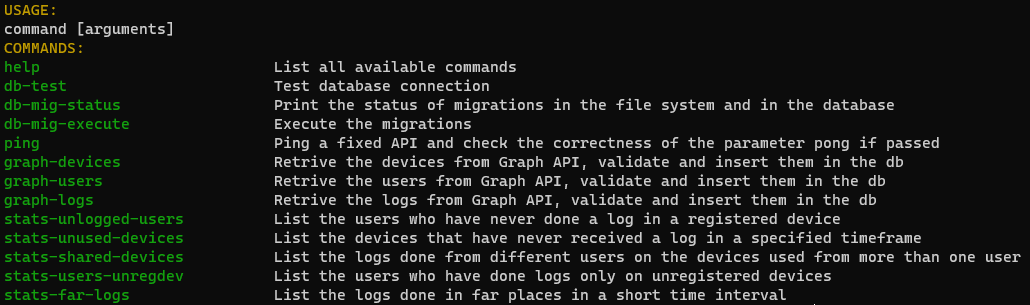
\includegraphics[width=\textwidth, height=7cm]{help-menu.png}
    \caption{help menu}
\end{figure}\\
Summing up, the main role of the console is to import all the required packages and execute the commands, through all the function contained in the other files.

\subsection{Configuration}
The parameters needed in the project, such as database information, API URLs, JSON files and other data files, are stored in the \texttt{config.ini} file. This allows the user to have a much more clear
overview of the possibility to change the information based on the current needs.\\
On the other hand this data are not directly contained in the Python code, so they need to be retrieved. The \texttt{ConfigParser} package comes in our help, allowing as to retrieve the data from the config file
and return them in any Python function.
\begin{python}
    def get_url():
        parser = ConfigParser()
        parser.read("config.ini")
        url = parser.get('ping', 'url')
        return url
\end{python}
The above code is an example of how the configuration function works. In the example, the parameter \texttt{url} is retrieved from the section \texttt{ping} of the \texttt{config.ini} file.

\subsection{Database Connection}
The first important step of the project was to set up a database. As said in the previous sections, the database was a PostgreSQL database, hosted in the Azure cloud.\\
One the database was up and running, the next step was to create a connection between the Python application and the database, in order to be able to store, modify and delete data directly from the application.\\
It twas chosen to use the \texttt{Psycopg2} library, which is the most popular PostgreSQL database adapter for the Python programming language. This package allows to open a connection, query the data, 
commit the changes and finally close the connection.
\begin{python}
    # parameters are host, database, user, password
    def connect(params):
        conn = None
        # connect to the PostgreSQL server
        conn = psycopg2.connect(**params)
        # create a cursor
        cur = conn.cursor()
        # execute a statement
        cur.execute('SELECT version()')
        # display the PostgreSQL database server version
        db_version = cur.fetchone()
        print(db_version)
        # close the communication with the PostgreSQL
        cur.close()
        return conn
\end{python}
The above code describe the \texttt{connect} function, that is one of the most fundamental functions of the project. It opens a connection with the database, then the \texttt{cursor} object allows to execute a query
and retrieve the result. Finally, the cursor is closed and the \texttt{conn} object is returned, in order to be used wherever is needed a database connection.

\subsection{Migrations}
\label{subsec:migrations}
During the development of the project the database was constantly modified: some tables was added, removed or altered. In order to keep track of all the changes, it was created a table named \texttt{migrations},
used to store the changes made to the database. The table is composed of two columns: the migration version and exact date and time of the entry insertion.\\
The concept of migrations was widely known in the company IT department, where the team makes a intense use of the \href{https://www.doctrine-project.org/projects/doctrine-migrations/en/3.3/index.html}{migration doctrine}, 
applied to PHP. In order to align my project with the company standards, it was chosen to use the concept of migrations. \\
There exist Python libraries useful to manage all the migrations, but since this is a small project, instead of learn the use of a complex library, it was chosen to personally develop the functions needed for the management 
of the database migrations.
\begin{figure}[h]
    \centering
    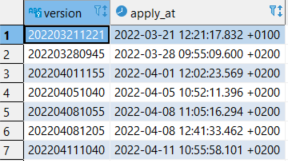
\includegraphics[width=8cm, height=4cm]{table-migrations.png}
    \caption{table migrations}
\end{figure}\\
Each time it was needed to modify the database, a SQL file was written and named with current date and time. Then it was checked if the instruction written into the file were ready to be applied to the 
database.\\
First it was checked if the name of the migration file respects the naming constraints, i.e., thanks to the \texttt{datetime} library, it was checked if the name was a valid date and time format.
The next step was to find out if the file was not already present in the database and if it was the most recent. If both conditions were verified, then the file was inserted in the \emph{ready to be executed}
list, meaning that the migrations was ready to be applied to the database.
\newline\newline\newline\newline
The main menu offers two migrations command:
\begin{itemize}
    \item \texttt{db-mig-status}: allows the user to have an overview of the migrations' status. It lists the migrations ready to be executed, the ones available only in the file system and those available
            only in the database. The last two are indicated as errors, since the file systems and the database migrations table must be aligned.
    \item \texttt{db-mig-execute}: execute all the migrations labelled as \emph{ready to be executed}. If the execution is successful the changes are committed to the database and a new entry is inserted in the
            migrations table. If the execution is not successful, the changes are rolled back and the user is informed.
\end{itemize}

\subsection{Azure Application}
\subsubsection{Azure Environment}
Azure is a cloud computing based platform for hosting applications and website, created and operated by Microsoft. After registering an application in the Azure portal, one can access and use all the services
provided by Microsoft Graph.
\subsubsection{Application Registration}
The project objective is to retrieve and analyze the data from Microsoft Graph. In order to be able to use this service, I had to register my application in the Azure portal.\\
Following the \href{https://docs.microsoft.com/en-us/graph/auth-v2-service#authentication-and-authorization-steps}{official documentation} and thanks to my company tutor support, the application was correctly
registered and the required permission was given. After the registration procedure, the application details were generated by the portal: client ID, secret, authority and scope. This data was saved in the 
\texttt{config.ini} file since they would be used soon to access the Microsoft Graph API.

\subsection{Microsoft Graph}
\subsubsection{Authorization and Connection}
Once the application was registered in Azure platform, in order to access the Microsoft Graph API, I had to connect my Python code to Microsoft Graph API. \\
Microsoft Azure makes use of \href{https://oauth.net/2/}{OAuth 2.0}, which is the industry-standard protocol for authorization, based on the concept of access tokens.\\
Authorization and connection was implemented following the \href{https://github.com/Azure-Samples/ms-identity-python-daemon/tree/master/1-Call-MsGraph-WithSecret}{official guide} and using the \texttt{msal} package.\\
Once the connection was established, an authentication token was generated, which is later used to access the Microsoft Graph API.
\begin{python}
  def connect(authority, client_id, scope, secret):
      app = msal.ConfidentialClientApplication(
            client_id, client_credential=secret, 
            authority=authority)
      result = app.acquire_token_silent(scope, account=None)
      if not result:
          result = app.acquire_token_for_client(scopes=scope)
      return result['access_token']
\end{python}
The above code snippet explains how the connection is established. The needed parameters are the client authority, ID, scope and secret. Then is checked if the token is still valid. If it is not, it is renewed
and at the end the token is returned and ready to be used to perform the requests to the Microsoft Graph API.

\subsubsection{Graph: Users}
The first set of data which I worked with is the list of all the users registered with a company Microsoft account.

\paragraph{Data Retrieval} ~\\
The first step was to retrieve the list of users from the Microsoft Graph API. The task was performed, as explained before, with a GET request, through the \texttt{requests} library.\\
An endpoint was needed and the one I used had the following url:  
\begin{Verbatim}[fontsize=\small]
https://graph.microsoft.com/v1.0/users?$top=999&$select=id,displayName
\end{Verbatim}
where the \texttt{\$select} parameter is used to retrieve only the fields needed.\\
The request is done inserting in the header the authorization token, whose importance was explained before. Finally, if the request was successful, the list of users is returned.

\paragraph{Response Validation} ~\\
Once the response of the endpoint was available, it needs to be validate, i.e., it must be checked that all the required fields are present and in the correct format.\\
The response of every API is a \texttt{json} text, so it is checked against a \texttt{json} file specifically written for the used endpoint. This is performed using the \texttt{validate} module of the 
\texttt{jsonschema} library.
The following snippet reports the \texttt{json} file written to check each object of response of the users endpoint:
\begin{python}
    {
    "id": {"type": "string"},
    "displayName": {"type": "string"},
    "required" : ["id"]
    }
\end{python}
It states that two fields are expected: \texttt{id} and \texttt{displayName} and both must be of string type, i.e., they must be a text. Moreover, the \texttt{required} instruction imposes that the \texttt{id} field
must be present, otherwise the validation will fail, while the \texttt{displayname} may be absent.\\
This \texttt{required} instruction was specified for the \texttt{id} since it will later be used a primary key in the database, so it cannot be a null value.

\paragraph{Database Insertion} ~\\
Finally, after the data was retrieved and validated, they are ready to be inserted in the database.\\
Through a migration (see section \hyperref[subsec:migrations]{4.4} for further information) the table \texttt{users} was created, with the following characteristics:
\begin{figure}[h]
    \centering
    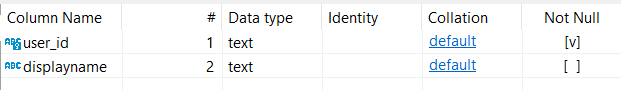
\includegraphics[width=10cm, height=2cm]{table-users.png}
    \caption{table users}
\end{figure}\\

One the users list is available, it must be inserted in the database. This is done though a cycle and for each entry of the list there are two possibilities:
\begin{itemize}
    \item \texttt{insert}. This command insert a user in the table if and only if the user is not already present in the table.
    \item \texttt{update}. If the user is already present in the table, this command updates the user's information.
\end{itemize}
FInally, at the end of the cycle, the changes to the database are committed and the connection is closed.

\newpage
\subsubsection{Graph Devices}
The second big set of data used in the project was the list of the company devices given to the employees.

\paragraph{Data Retrieval} ~\\
Such as for the users, first step was to retrieve the list of devices from the Microsoft Graph API. The task was performed, with a GET request, through the \texttt{requests} library.\\
An endpoint was needed and the one I used had the following url:  
\begin{Verbatim}[fontsize=\small]
https://graph.microsoft.com/v1.0/devices?$top=999&$select=deviceID,
id,displayName,registrationDateTime,approximateLastSignInDateTime
\end{Verbatim}
where again the \texttt{\$select} parameter is used to retrieve only the fields needed.

\paragraph{Data Validation} ~\\
In the same way as it was explained before, the response of the endpoint was validated, i.e., checked against a \texttt{json} file specifically written for the used endpoint.\\
The following piece of code shows an extract of the \texttt{json} file:
\begin{python}
{
...
"registrationDateTime": {"type": "DateTimeOffset"},
"approximateLastSignInDateTime": {"type": "DateTimeOffset"},
"required" : ["deviceId", "id", "displayName"]
}
\end{python}
The deviceID, id and displayname fields are omitted since they are \texttt{string} and there are no differences with respect to what explained for the user \texttt{json} file.
What is new are the \texttt{registrationDateTime} and \\ \texttt{approximateLastSignInDateTime} fields, which are dates and are expressed as \texttt{DateTimeOffset} format.

\paragraph{Active Devices} ~\\
The problem of the devices list retrieved from Microsoft Graph is that it contains not only the active devices, but also the devices that are not active anymore, such as old notebooks or phones.
In order to overcome this problem, the devices list was filtered to obtain only the devices effectively active in a time period, determined in the \texttt{config.ini} file.\\
After the validation the two date fields were converted in \texttt{date object}, fundamental for working with dates in Python. Then, the devices list was filtered to obtain only the devices that are active 
in the desired period.\\
The following code explains how the list of the active devices is obtained:
\begin{python}
def list_active_devices(devices, active_period):
   today = datetime.now()
   start_date = (
      today -
      timedelta(
         days=active_period,
         hours=today.hour,
         minutes=today.minute,
         seconds=today.second)).strftime("%Y-%m-%dT%H:%M:%SZ")
   active_devices = []
   for device in devices:
       last_login = device['approximateLastSignInDateTime']
       if last_login is not None and last_login >= start_date:
           active_devices.append(device)
   return active_devices
\end{python}
First the start date is found, subtracting the number of days specified in the period from the current date, thanks to the \texttt{timedelta} function. The obtained date is converted in a date object using the
\texttt{strftime} function.\\
Then, the list of devices is cycled and only the devices with a last login more recent than the start date are added to the list of active devices, that is in the end returned.\\
At the end of the function, we will have a list containing only the devices with the last login done in a defined time period.

\paragraph{Database insertion and deletion} ~\\
Finally, the list of active devices is inserted in the database. The process is similar to the one for the users.\\
The table \texttt{devices} was created, with the following characteristics:
\begin{figure}[h]
    \centering
    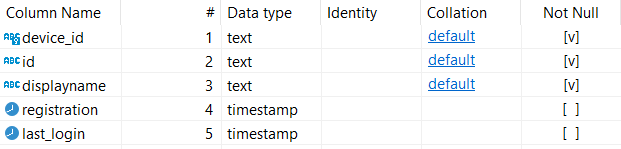
\includegraphics[width=12cm, height=3cm]{table-devices.png}
    \caption{table devices}
\end{figure}\\
The main difference with respect to the users part is that the devices stores in the database must be deleted once they exit the active period.
\newline\newline
This simple piece of code solve the problem:
\begin{python}
    for device in devices:
        ...
        cur.execute(sql_check, (deviceID,))
        if cur.fetchone()[0] is False:
            insert(cur, deviceID, id, name, date, last_login)
        else:
            update(cur, deviceID, last_login)
    delete_devices(cur, active_period)
    ...
\end{python}
It checks, for each device in the list, if it is already present in the database. If it is not present, it is inserted, otherwise the device information are updated. At the end of the cycle, 
the devices that are not active anymore are deleted.

\subsubsection{Graph: Logs}
The most important and complex set of data was the list of all the logs done by every employee.

\paragraph{Data Retrieval} ~\\
The most complicated task of this part of the project was to retrieve the list of all logs from Microsoft Azure, since Graph allows to retrieve at most 1000 entry at single HTTP request. To overcome this problem
successive requests were made. The paging system of Azure was managed included the authentication token for the next request in the header of the previous API response, when the next token field was missing it means
that it was the last page.\\
Moreover it was asked to retrieve only the logs done in a specified period, whose values was specified in the \texttt{config.ini} file.
\begin{python}
    ...
    while next_link is not None:
        print("Retrieving information from Azure")
        logs = requests.get(next_link, headers=headers).json()
        insert_logs(conn, logs['value'], file_schema)
        if "@odata.nextLink" in logs:
            next_link = logs['@odata.nextLink']
        else:
            next_link = None
    ...
\end{python}
The above code reports how the paging issue was solved: each time a page is returned, the \texttt{nextLink} is saved and used as URL for the next request.

\paragraph{Data Validation} ~\\
In the same way as explained in the preceding sections, the response of the endpoint was validated, i.e., checked against a \texttt{json} file specifically written for the used endpoint.\\
After the validation, all the date fields were converted in \texttt{date object}, in order to be ready to be used and inserted in the database.

\paragraph{Database insertion} ~\\
FIrst the table logs was created, with the following structure:
\begin{figure}[h]
    \centering
    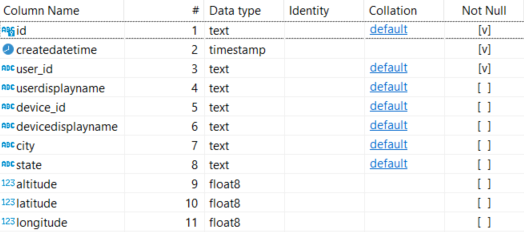
\includegraphics[width=13cm, height=5.5cm]{table-logs.png}
    \caption{table logs}
\end{figure}\\
Since the logs were retrieved up to a defined number of days and the script may be run everyday, only the new logs had to be inserted in the database. To achieve this result, each entry of the retrieved list 
was checked against the rows of the db. If the record is not found in the database it is inserted, otherwise it is ignored.

\subsection{Docker}
After all the code development described in the previous sections, the script was ready and able to retrieve, validate and insert the data in the database.\\
At this point the only problem was that the project was developed on a specific Windows machine, so every command needed to be executed from that machine in order to be able to run properly.\\
This was a problem since the script needed to be run from any machines, including servers and Unix environments. To overcome this issue, the whole project was packaged in a Docker container, which
create an environment that could be run in every device.\\
First I had to learn how to use the Docker technology, then I installed Docker Desktop, which is a graphic interface for create and managing docker container. Once I was ready, I created a docker container for
my project and I wrote the needed \texttt{Dockerfile}. \\
The \texttt{Dockerfile} is the instruction file needed to correctly setup the Docker environment and inside the following parameters was specified:
\begin{itemize}
    \item \textbf{Python}: it was specified which version of Python to use and the standard path of Python in a generic machine.
    \item \textbf{Packages}: the needed packaged for the project were listed in order to be installed inside the Docker container.
    \item \textbf{Entrypoint}: using bash instructions, there were specified which commands to execute when the container is started.
\end{itemize}
Once the container was ready, it was possible to run the wanted script from every device.\\
In our case, the commands specified in the \texttt{Entrypoint} were the ones to retrieve, validate and insert aal the needed data in the database. At the end only one command was run:
\begin{center}
\scriptsize
\begin{BVerbatim}
docker run --rm -it --name python-dev-container -p 1010:1010 python-dev-image  
\end{BVerbatim}
\end{center}
as a consequence of this command the database was populated with the users, devices and logs data.\\
In the end after the Docker technology was applied to the project, it could be run from any machine and with a single command, all the operations for retrieve the data and populate the database would be executed. 

\subsection{Data Analysis}
Data analysis and the creation of statistics about the available data was the final objective of the project.\\
There were performed five main analysis:
\begin{enumerate}
    \item Users who have never done a login with their company account
    \item Company devices which have never received a login
    \item Company devices which are shared with more than one employee
    \item Users who hav done login only in unregistered devices (i.e., devices that are not in the database)
    \item Consecutive logs done by the same user in a short amount of time in two different and far locations 
\end{enumerate}
\newpage
Each of the analysis described have a correspondent command in the console menu. Those commands can be execute with an additional optional parameter which specifies the time duration in which the analysis is performed.
If the parameter is not inserted the default interval is ninety days from the current date. 

\subsubsection{Analysis creation}
All the statistics listed before were realized twice: first they were created using only standard SQL without any extension, i.e., each statistic was a single query whose complexity varied from one to the other.\\
SQL is an achromic for \texttt{Structured Query Language}, which is a standardized language that is used to interrogate relational databases.\\
In a second moment everything done in SQL was realized again using Python, i.e., integrating Python coding with more simple queries to the database.\\
In this section there will not be any code, but all the SQL and Python files can be find in the \href{https:\\github.com}{project repository}.

\subsubsection{Unlogged users}
The first analysis create was the one dedicated to find all the employees who have never done a login with their company account.\\
In order to select only the users who have never logged in, it was needed to select the list of users present in the table \texttt{users} and not present in the table \texttt{logs}.\\
Initially it was though to use the \texttt{NOT EXISTS} or the \texttt{EXCEPT} operator, that as the names suggest select the entry available in a table and not in the other one.
However, it was found out that these two methods are not very efficient, so it was finally choses to adopt the \texttt{LEFT JOIN} operator, which is a kind of join operator which selects the rows of the 
first table that are not present in the second one. By adopting the join operator, the efficiency of the query incredibly increased.\\
Since the query was a very simple one, the Python implementation was simply the code needed to run the query.\\
At the end, after running the correspondent command of this analysis, the \texttt{id} and \texttt{displayName} of the selected users were shown as result.

\newpage
\subsubsection{Unused devices}
In a second moment it was necessary to create a second analysis, similar to the first one, but regarding the devices. It was indeed needed to find all the devices that have never received a login.\\
The procedure was similar to the one adopted in the first analysis, so we needed to select only the devices available in the table \texttt{devices} and not in the table \texttt{logs}.\\
Since the query was similar to the previous one, it was directly done using the \texttt{LEFT JOIN} to select only the rows present in the first table and not in the second one.\\
Once again the Python implementation was only the code needed to run the query.\\
At the end, after running the correspondent command, the \texttt{id} and \texttt{displayName} of the selected devices were shown as result.

\subsubsection{Shared devices}
\label{subsubsec:shared}
The third analysis is the one that was created to find all the devices that are shared with more than one employee and all the login done on those devices.\\
This was a more complex query, since more data manipulations were needed before the expected result could be selected.\\
Itt was needed to select from the logs table only the logs done on devices which had received login from more than one different users.\\
Firs it was created a subquery in order to select from the table \texttt{logs} the \texttt{id} of the devices on which have been done access from more than one user.\\ 
Then the result of the subquery was joined with the table \texttt{logs} in order to select only the logs of the devices whose id was selected before. Finally the result was grouped using the \texttt{group by}
statement, in order to have not repeated logs done from the same user on the same device. As last step the list of the selected logs was ordered, through the \texttt{order by} operator to have a more 
readable result.\\  
This analysis was more complex with respect to the previous one, but once the logic of the query was learned, everything could be easily written in SQL language.
For this reason the Python implementation is, once again, the simple code needed to run a SQL query.\\
At the end, the result of the main menu command shows the \texttt{id} and \texttt{displayName} of the shared devices and the \texttt{id} and \texttt{displayName} of the users who have done login on them.

\subsubsection{Logs on unknown devices}
\label{subsubsec:unknown}
This statistics was created to find all the users who have done login only on devices not registered in the company system.\\
First it was needed a subquery to find all the entries from the table \texttt{logs} with the column \texttt{deviceId} equal to \texttt{NULL}, i.e., all the logs done on an unknown device.\\
Then the table \texttt{users} was joined with the table \texttt{logs} in order to have information about both users and logs. From the result of this join operation, there were selected only the rows present
in the result of the subquery previously written. By doing this we have obtained only the entries corresponding to the logs done on unknown devices.\\
Finally, it was required to return information about the users who have done those logs, so from the final result, only the columns \texttt{userID} and \texttt{userDisplayname} were selected.\\
The result of the command correspondent to this analysis are the \texttt{id} and \texttt{displayName} of the users who have done login on unknown devices.\\
Once again the Python implementation is the simple code needed to run the corresponding SQL query.

\subsubsection{Impossible logs}
\label{subsubsec:impossible}
The last analysis was realized to find all the logs there were physically impossible, i.e., the logs done in a short time interval and in two different and far location.
For example two successive logs done from the same user in a time interval of two minutes and in two location 100 km apart. This example is clearly an impossible log, since it is not possible to travel 100 km
in only two minutes.\\
In the \texttt{logs} table, the position of a specific log is given by the latitude and longitude of the device on which the log was done.\\
PostgreSQL offers an additional module called PostGIS, which is a module that allows to perform spatial queries on the database. This extension is complex and it is used when very precises measurements are
needed.\\
Since it was decided to use only standard SQL and a precise measurement was not needed for the purpose of the analysis, it was chosen to directly calculate the distances between the two points, using the
\href{https://en.wikipedia.org/wiki/Haversine_formula}{Haversine formula}:
\[
    d = 2r\arcsin \left( \sqrt{ \sin^2\left(\frac{\varphi_2 - \varphi_1} {2}\right) + \cos(\varphi_1)\cdot\cos(\varphi_2) \cdot \sin^2\left(\frac{\lambda_2 - \lambda_1} {2}\right) } \right)
\]
where $\varphi_1, \varphi_2$ are the latitude and $\lambda_1, \lambda_2$ the longitude of the two points and \emph{r} is the radius of the earth.\\
Since the query needed for this analysis was quite complex, all the calculations were divided among Python and SQL.
First it was created a materialized view, which is a view that is stored in the database.\\ Its purpose is to store all the data of the table \texttt{logs}, adding four new columns:
\begin{itemize}
    \item \texttt{prec\_time}, which is the time of the previous log done from the same user
    \item \texttt{time\_diff}, which is the time difference between the time of the previous and the current log
    \item \texttt{prec\_lat}, which is the latitude of the previous log done from the same user
    \item \texttt{prec\_long}, which is the longitude of the previous log done from the same user
    \item \texttt{dist\_diff}, which is the distance difference between the location of the previous and the current log
\end{itemize}
The creation of this materialized view was by far the most difficult part of the analysis since the complex formula previously described was needed to be written
in SQL language. Moreover, in order to calculate the time difference and the distance difference, it was required to access two entries of the table \texttt{logs}, so that
the selected logs were consecutive and done by the same user. \\
This was not an easy task since in standard SQL is not possible to execute cycles in a query. To overcome this difficulty, I made use of the \texttt{lag}
Window function. Window functions allow to partition and order the table with respect to a specific column of the table. In our case the logs were partitioned
by \texttt{user\_id} ordered by \texttt{createDatetime} in order to access in a consecutive way only the logs done by the same user.\\
Once the materialized view was created, I performed the remaining calculation using Python. First the time period and the distance used to select the impossible
logs were retrieved by the \texttt{config.ini} file. The a simple SQL query was written in order to select from the materialized view only the entries whose 
\texttt{dist\_diff} and \texttt{time\_diff} are respectively greater and smaller than the values specified in the \texttt{config.ini} file.\\
At this point all the impossible logs, i.e. the logs done in a time interval shorter than the one required and with a distance between the two points greater than the one specified,
had been found.\\
Finally all the columns of the materialized view were selected in order to give to the user all the information about those impossible logs and about the users
who have performed them.

\subsection{Report Creation}
The final part of the project was to create visual reports of all the analysis described in the previous section.\\
The software used to create those report is Power Bi, which is an interactive data visualization software product developed by Microsoft. Power BI is a collection of software services,
apps, and connectors that work together to turn unrelated sources of data into coherent, visually immersive, and interactive insights.
In our case the data source was the database, which was indeed connected to Power Bi. \\
The peculiarity and great advantage of this software is that it allows to import the data and store an internal copy. Then these data may be manipulated while the original copy in the database is not
subject to any modification.\\
Since I was new to this technology, I was given the possibility to follow a one day workshop about Power Bi, directly organized by a Microsoft partner company called BitBang. Thanks to this informative
session, I learned the basis of the software. Successively I keep learning in order to be able to create clean and understandable reports.

\paragraph{Informations} ~\\
This section will be rich of images, since I think it is not possible to describe graphic reports without the use of images of the reports themselves. \\
All the captions in the reports will be in italian, since Ubroker is an italian company and I was asked to write in italian.\\
Moreover the images will have some censured parts, since the reports include private information about the employee that, for privacy issues, cannot be shown in a public document.

\subsubsection{Data Source}
The original data source was the database previously described, with the table \texttt{users}, \texttt{devices} and \texttt{logs}. Moreover some other view were created, in order to ease the creation of the
reports.\\
In addition to what was present in the database, some table was also created inside Power Bi. using his own language, called DAX which is a collection of functions, operators, and constants that can be used 
in a formula, or expression, to calculate and return one or more values. For example the join of two table was one of the simple actions executed using DAX.

\newpage
\subsubsection{Logs Overview}
The first report was created to show an overview of the logs done, showing the number of login per each day, the users who have done them and the devices used. Moreover a map of the logs location is shown as
well.
\begin{figure}[h]
    \centering
    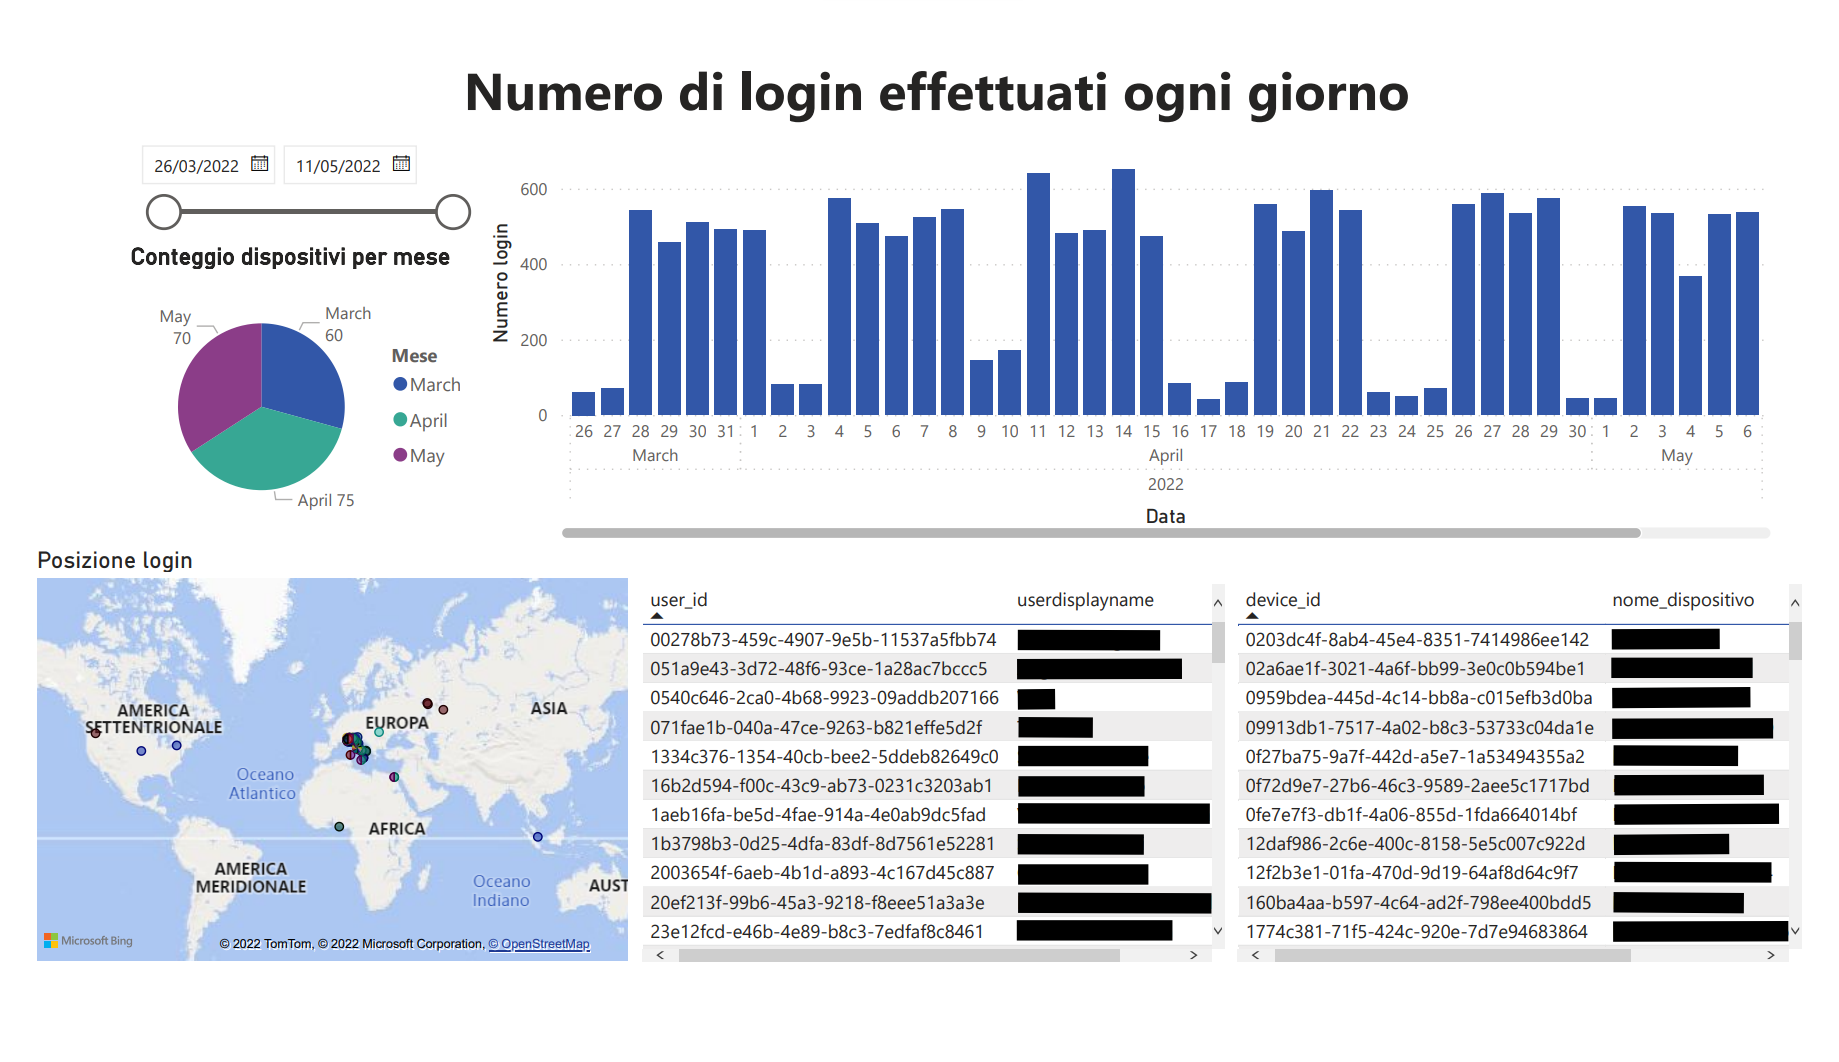
\includegraphics[width=\textwidth, height=8cm]{log-per-day.png}
    \caption{logs per day report}
\end{figure}\\
The above image represent the first report, which gives information about the logs done each day. It is composed by several visual element, i.e., the object used in Power Bi to realize the report.\\
The first most outstanding visual element is an histogram, which shows the number of login per each day, then there are two table, which show the users who have done the login and the devices used.\\
There is then a map of the logs and a slicer, which allows to select the time period of the logs to be shown.\\
The peculiarity of a Power Bi reports, which is not visible through an image, is its dynamism. Each time we interact with an object, we modifies the other ones too, for example if we select a single day from the
histogram, the two tables will show only the users and the devices interested in that day. The map will be show the location of the logs of the selected day only.\\
This mechanism works also the other day, if we select a user then the report will show only the information regarding the selected employee.\\

\subsubsection{Users and Devices}
The aim of these reports is to create a visual representation of the result of the analysis described in the precedent section. \\
In order to represent all the analysis reports about the devices which have never received a login and users who have never done a login were created as well.\\
This two reports were created using DAX language to join the tables directly inside Power Bi and avoiding the creation of two additional views in the database.\\
No images about those two reports will be inserted, since they both consist of a table, a slice to select the time period and a counter to show the results numbers.

\subsubsection{Shared Devices}
This report is another important one, since it shows the devices that have been shared by the users.
\begin{figure}[h]
    \centering
    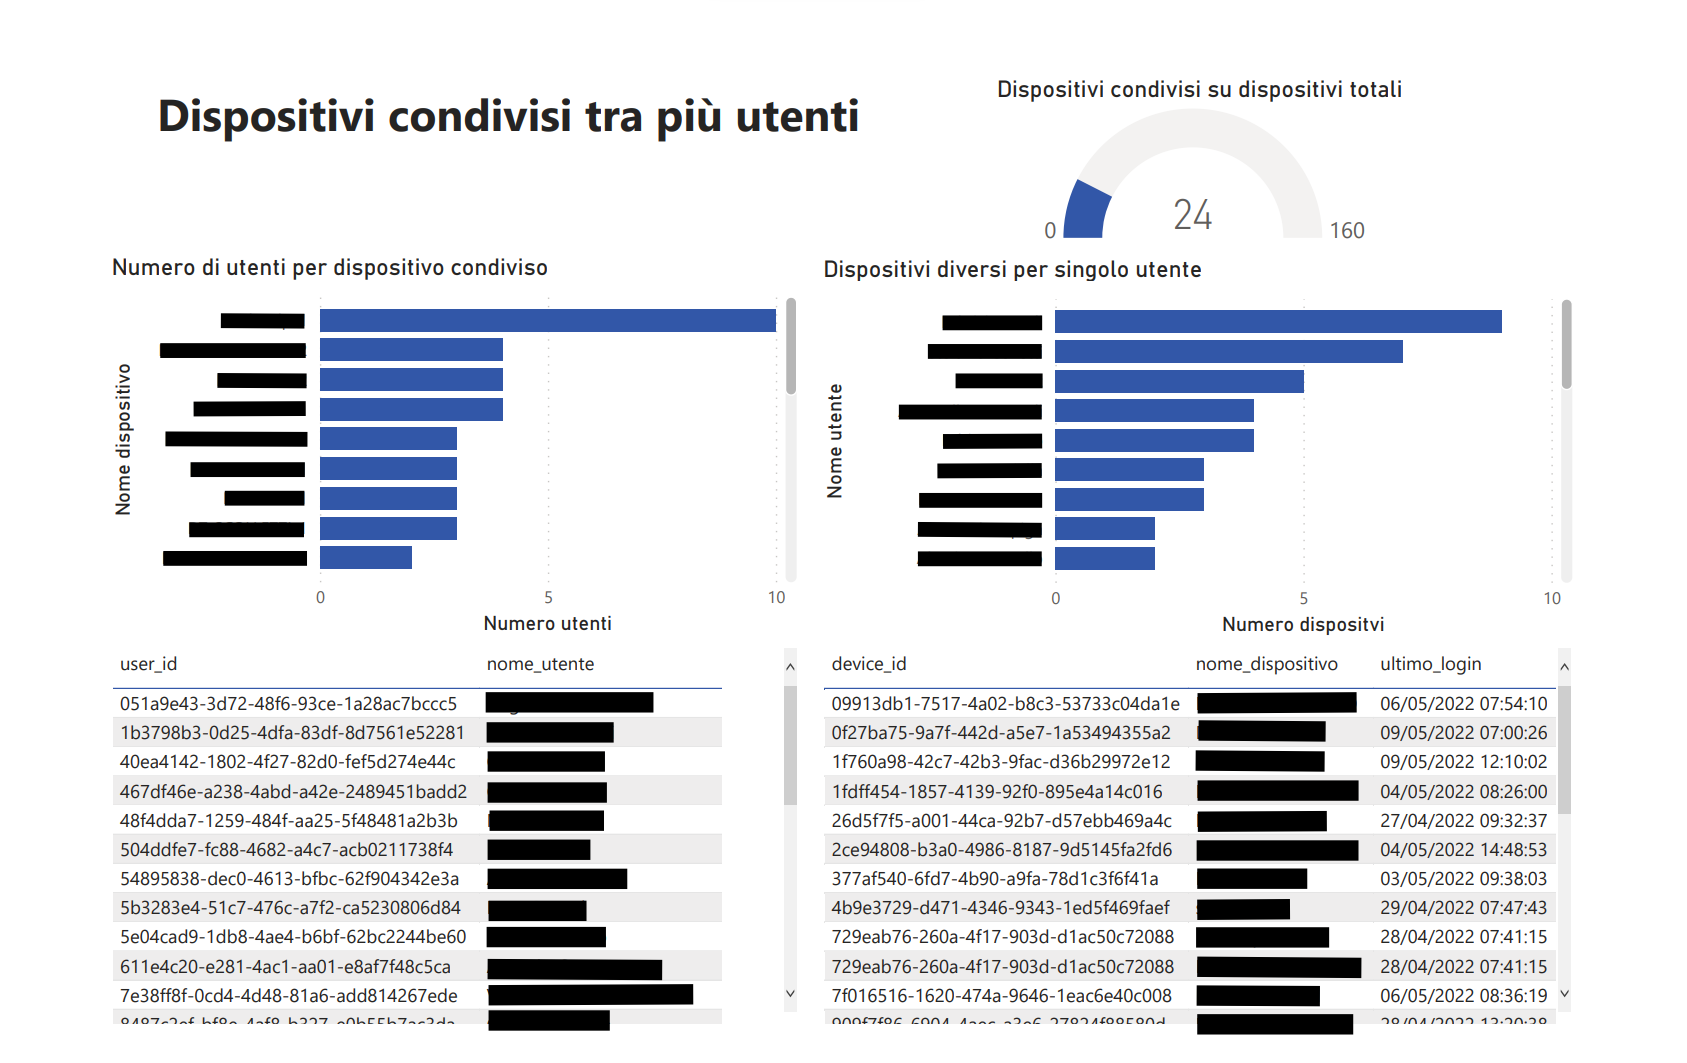
\includegraphics[width=\textwidth, height=8cm]{shared-devices.png}
    \caption{shared devices report}
\end{figure}\\
This model is composed by two vertical bar chart: the left one shows the number of users for a shared devices, while the one on the right shows the number of shared devices for each user.
There are then \texttt{users} and \texttt{devices} tables, used to show the list of users and devices included in the report. \\
Last a counter is used to show how many devices are shared with respect to the total number.
To create this report, it was necessary to create a view in the database, since it was too difficult to express a complex query in DAX language. The created view is the result of the query explained in 
\hyperref[subsubsec:shared]{4.8.4} section, which is then memorized and used to build the final report.

\subsubsection{Users with logs on unknown devices}
In this section it will be described the report that shows the users that have done a login on unknown devices. \\
Similarly to the previous one, to realize this report, it was previously created a view in the database, which is the result of the query explained in \hyperref[subsubsec:unknown]{4.8.5} section.\\
Once the view was ready, it was imported in Power Bi and used as data source. This specific report has not any new visual element with respect to the previous ones. It is indeed composed by a table which
shows the users who have done logs only on devices not registered in the company database.
There is a then a slicer to select the time period of the logs to be shown, a counter which shows the users count and finally an histogram which reports the number of login on unknown devices done each day.

\subsubsection{Impossible Logs}
The last report is the one representing the impossible logs analysis. That analysis was the most difficult one, consequently the report was difficult too.\\
The report is composed by three page, all showing different aspects of the logs impossible to be done. The realization of those three pages required the creation of two views in the database: one containing
all the logs with with the fields \texttt{dist\_diff} and \texttt{time\_diff} and the other one containing only the couples of impossible logs, which is basically the result of the analysis explained in
\hyperref[subsubsec:impossible]{4.8.6} section.\\
In the next page it is shown an image of the first page of this report, which is composed by a table showing all the impossible logs and highlighting the time interval and the distance difference between two
consecutive logs. There is then a bar chart showing the users who have done these logs and how many times they have done them. Finally it was inserted an histogram to show how many impossible logs were done
every day.
\newline\newline\newline\newline
\begin{figure}[h]
    \centering
    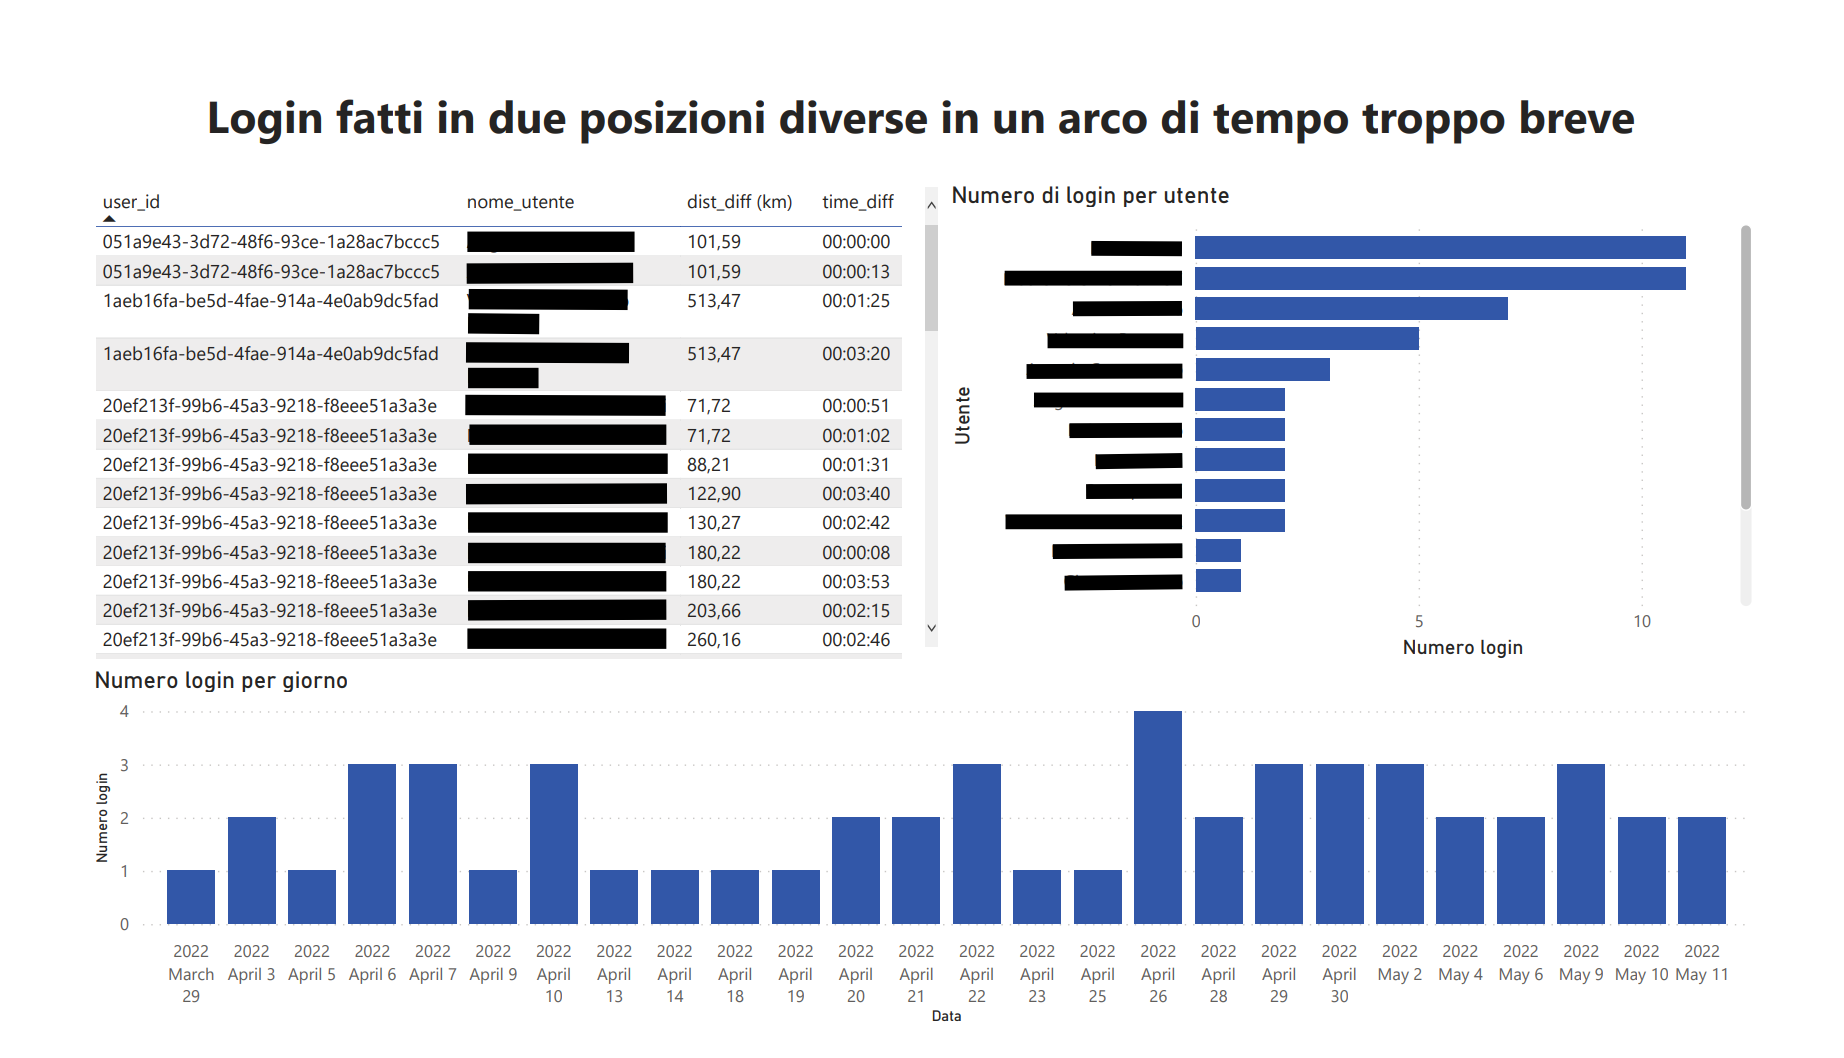
\includegraphics[width=\textwidth, height=8cm]{impossible-logs.png}
    \caption{impossible logs report}
\end{figure}\\
The second page of the report is composed by two maps showing the location of a couple of impossible logs and by an object showing the date and time of the log reported in the map.\\
The two pages of the report are connect, i.e., thanks to a functionality called \emph{drill through}, we can select a log from the table in the first page and in the second page will be shown the position
of the selected log and the preceding one.\\
In the third and last page of the report, it was required to have the possibility to select from a table with all the logs only the ones that are or are not possible. To fulfil the request, the view containing
all the logs, was modified using DAX language and a column \texttt{validity} was added to the table, this new column may assume only two values: yes or no.\\
specifically the last page is composed by a table, with the added column, a filter used to selected the wanted logs and by a bar chart that, similarly to the one in the first page, shows the logs count per user.

\newpage
\section{Conclusion and Considerations}



\end{document}